\pdfinfoomitdate=1
\pdftrailerid{}
\pdfsuppressptexinfo=-1
\documentclass[border=6pt]{standalone}
\usepackage{amsmath,amssymb}
\usepackage{tikz}
\usetikzlibrary{arrows.meta,decorations.pathreplacing,positioning}
\begin{document}
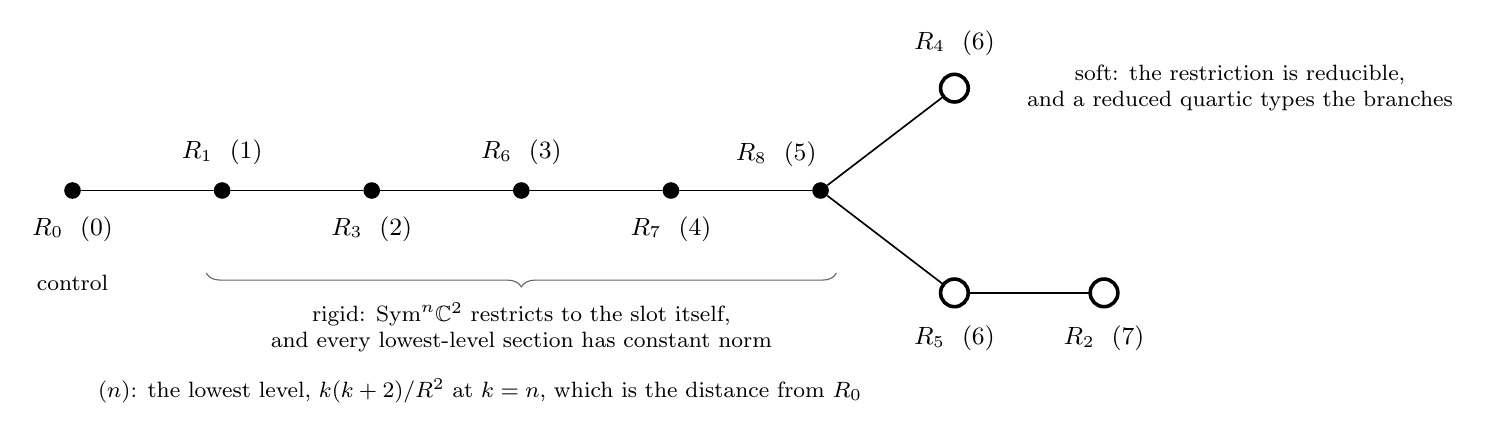
\begin{tikzpicture}[line cap=round, line join=round,
  soft/.style={circle, draw, line width=1.3pt, fill=white, minimum size=10pt, inner sep=0pt},
  rigid/.style={circle, fill, minimum size=6pt, inner sep=0pt}]
\node[rigid] (R0) at (0.00,0.00) {};
\node[rigid] (R1) at (1.90,0.00) {};
\node[rigid] (R3) at (3.80,0.00) {};
\node[rigid] (R6) at (5.70,0.00) {};
\node[rigid] (R7) at (7.60,0.00) {};
\node[rigid] (R8) at (9.50,0.00) {};
\node[soft] (R4) at (11.20,1.30) {};
\node[soft] (R5) at (11.20,-1.30) {};
\node[soft] (R2) at (13.10,-1.30) {};
\draw[semithick] (R0) -- (R1);
\draw[semithick] (R1) -- (R3);
\draw[semithick] (R3) -- (R6);
\draw[semithick] (R6) -- (R7);
\draw[semithick] (R7) -- (R8);
\draw[semithick] (R8) -- (R4);
\draw[semithick] (R8) -- (R5);
\draw[semithick] (R5) -- (R2);
\node[below=5pt of R0, font=\small, inner sep=1pt] {$R_0$ \ (0)};
\node[above=5pt of R1, font=\small, inner sep=1pt] {$R_1$ \ (1)};
\node[below=5pt of R3, font=\small, inner sep=1pt] {$R_3$ \ (2)};
\node[above=5pt of R6, font=\small, inner sep=1pt] {$R_6$ \ (3)};
\node[below=5pt of R7, font=\small, inner sep=1pt] {$R_7$ \ (4)};
\node[above left=5pt and -2pt of R8, font=\small, inner sep=1pt] {$R_8$ \ (5)};
\node[above=5pt of R4, font=\small, inner sep=1pt] {$R_4$ \ (6)};
\node[below=5pt of R5, font=\small, inner sep=1pt] {$R_5$ \ (6)};
\node[below=5pt of R2, font=\small, inner sep=1pt] {$R_2$ \ (7)};
\node[font=\footnotesize, anchor=north] at (0,-0.95) {control};
\draw[decorate, decoration={brace, amplitude=5pt, mirror}, black!60] (1.70,-1.05) -- (9.70,-1.05);
\node[font=\footnotesize, align=center, anchor=north] at (5.70,-1.30) {rigid: $\mathrm{Sym}^{n}\mathbb{C}^2$ restricts to the slot itself,\\ and every lowest-level section has constant norm};
\node[font=\footnotesize, align=center, anchor=west] at (12.0,1.30) {soft: the restriction is reducible,\\ and a reduced quartic types the branches};
\node[font=\footnotesize, anchor=west] at (0.2,-2.55) {$(n)$: the lowest level, $k(k+2)/R^2$ at $k = n$, which is the distance from $R_0$};
\end{tikzpicture}
\end{document}
